% Options for packages loaded elsewhere
\PassOptionsToPackage{unicode}{hyperref}
\PassOptionsToPackage{hyphens}{url}
\PassOptionsToPackage{dvipsnames,svgnames,x11names}{xcolor}
%
\documentclass[
  letterpaper,
  DIV=11,
  numbers=noendperiod]{scrartcl}

\usepackage{amsmath,amssymb}
\usepackage{iftex}
\ifPDFTeX
  \usepackage[T1]{fontenc}
  \usepackage[utf8]{inputenc}
  \usepackage{textcomp} % provide euro and other symbols
\else % if luatex or xetex
  \usepackage{unicode-math}
  \defaultfontfeatures{Scale=MatchLowercase}
  \defaultfontfeatures[\rmfamily]{Ligatures=TeX,Scale=1}
\fi
\usepackage{lmodern}
\ifPDFTeX\else  
    % xetex/luatex font selection
\fi
% Use upquote if available, for straight quotes in verbatim environments
\IfFileExists{upquote.sty}{\usepackage{upquote}}{}
\IfFileExists{microtype.sty}{% use microtype if available
  \usepackage[]{microtype}
  \UseMicrotypeSet[protrusion]{basicmath} % disable protrusion for tt fonts
}{}
\makeatletter
\@ifundefined{KOMAClassName}{% if non-KOMA class
  \IfFileExists{parskip.sty}{%
    \usepackage{parskip}
  }{% else
    \setlength{\parindent}{0pt}
    \setlength{\parskip}{6pt plus 2pt minus 1pt}}
}{% if KOMA class
  \KOMAoptions{parskip=half}}
\makeatother
\usepackage{xcolor}
\setlength{\emergencystretch}{3em} % prevent overfull lines
\setcounter{secnumdepth}{-\maxdimen} % remove section numbering
% Make \paragraph and \subparagraph free-standing
\makeatletter
\ifx\paragraph\undefined\else
  \let\oldparagraph\paragraph
  \renewcommand{\paragraph}{
    \@ifstar
      \xxxParagraphStar
      \xxxParagraphNoStar
  }
  \newcommand{\xxxParagraphStar}[1]{\oldparagraph*{#1}\mbox{}}
  \newcommand{\xxxParagraphNoStar}[1]{\oldparagraph{#1}\mbox{}}
\fi
\ifx\subparagraph\undefined\else
  \let\oldsubparagraph\subparagraph
  \renewcommand{\subparagraph}{
    \@ifstar
      \xxxSubParagraphStar
      \xxxSubParagraphNoStar
  }
  \newcommand{\xxxSubParagraphStar}[1]{\oldsubparagraph*{#1}\mbox{}}
  \newcommand{\xxxSubParagraphNoStar}[1]{\oldsubparagraph{#1}\mbox{}}
\fi
\makeatother

\usepackage{color}
\usepackage{fancyvrb}
\newcommand{\VerbBar}{|}
\newcommand{\VERB}{\Verb[commandchars=\\\{\}]}
\DefineVerbatimEnvironment{Highlighting}{Verbatim}{commandchars=\\\{\}}
% Add ',fontsize=\small' for more characters per line
\usepackage{framed}
\definecolor{shadecolor}{RGB}{241,243,245}
\newenvironment{Shaded}{\begin{snugshade}}{\end{snugshade}}
\newcommand{\AlertTok}[1]{\textcolor[rgb]{0.68,0.00,0.00}{#1}}
\newcommand{\AnnotationTok}[1]{\textcolor[rgb]{0.37,0.37,0.37}{#1}}
\newcommand{\AttributeTok}[1]{\textcolor[rgb]{0.40,0.45,0.13}{#1}}
\newcommand{\BaseNTok}[1]{\textcolor[rgb]{0.68,0.00,0.00}{#1}}
\newcommand{\BuiltInTok}[1]{\textcolor[rgb]{0.00,0.23,0.31}{#1}}
\newcommand{\CharTok}[1]{\textcolor[rgb]{0.13,0.47,0.30}{#1}}
\newcommand{\CommentTok}[1]{\textcolor[rgb]{0.37,0.37,0.37}{#1}}
\newcommand{\CommentVarTok}[1]{\textcolor[rgb]{0.37,0.37,0.37}{\textit{#1}}}
\newcommand{\ConstantTok}[1]{\textcolor[rgb]{0.56,0.35,0.01}{#1}}
\newcommand{\ControlFlowTok}[1]{\textcolor[rgb]{0.00,0.23,0.31}{\textbf{#1}}}
\newcommand{\DataTypeTok}[1]{\textcolor[rgb]{0.68,0.00,0.00}{#1}}
\newcommand{\DecValTok}[1]{\textcolor[rgb]{0.68,0.00,0.00}{#1}}
\newcommand{\DocumentationTok}[1]{\textcolor[rgb]{0.37,0.37,0.37}{\textit{#1}}}
\newcommand{\ErrorTok}[1]{\textcolor[rgb]{0.68,0.00,0.00}{#1}}
\newcommand{\ExtensionTok}[1]{\textcolor[rgb]{0.00,0.23,0.31}{#1}}
\newcommand{\FloatTok}[1]{\textcolor[rgb]{0.68,0.00,0.00}{#1}}
\newcommand{\FunctionTok}[1]{\textcolor[rgb]{0.28,0.35,0.67}{#1}}
\newcommand{\ImportTok}[1]{\textcolor[rgb]{0.00,0.46,0.62}{#1}}
\newcommand{\InformationTok}[1]{\textcolor[rgb]{0.37,0.37,0.37}{#1}}
\newcommand{\KeywordTok}[1]{\textcolor[rgb]{0.00,0.23,0.31}{\textbf{#1}}}
\newcommand{\NormalTok}[1]{\textcolor[rgb]{0.00,0.23,0.31}{#1}}
\newcommand{\OperatorTok}[1]{\textcolor[rgb]{0.37,0.37,0.37}{#1}}
\newcommand{\OtherTok}[1]{\textcolor[rgb]{0.00,0.23,0.31}{#1}}
\newcommand{\PreprocessorTok}[1]{\textcolor[rgb]{0.68,0.00,0.00}{#1}}
\newcommand{\RegionMarkerTok}[1]{\textcolor[rgb]{0.00,0.23,0.31}{#1}}
\newcommand{\SpecialCharTok}[1]{\textcolor[rgb]{0.37,0.37,0.37}{#1}}
\newcommand{\SpecialStringTok}[1]{\textcolor[rgb]{0.13,0.47,0.30}{#1}}
\newcommand{\StringTok}[1]{\textcolor[rgb]{0.13,0.47,0.30}{#1}}
\newcommand{\VariableTok}[1]{\textcolor[rgb]{0.07,0.07,0.07}{#1}}
\newcommand{\VerbatimStringTok}[1]{\textcolor[rgb]{0.13,0.47,0.30}{#1}}
\newcommand{\WarningTok}[1]{\textcolor[rgb]{0.37,0.37,0.37}{\textit{#1}}}

\providecommand{\tightlist}{%
  \setlength{\itemsep}{0pt}\setlength{\parskip}{0pt}}\usepackage{longtable,booktabs,array}
\usepackage{calc} % for calculating minipage widths
% Correct order of tables after \paragraph or \subparagraph
\usepackage{etoolbox}
\makeatletter
\patchcmd\longtable{\par}{\if@noskipsec\mbox{}\fi\par}{}{}
\makeatother
% Allow footnotes in longtable head/foot
\IfFileExists{footnotehyper.sty}{\usepackage{footnotehyper}}{\usepackage{footnote}}
\makesavenoteenv{longtable}
\usepackage{graphicx}
\makeatletter
\def\maxwidth{\ifdim\Gin@nat@width>\linewidth\linewidth\else\Gin@nat@width\fi}
\def\maxheight{\ifdim\Gin@nat@height>\textheight\textheight\else\Gin@nat@height\fi}
\makeatother
% Scale images if necessary, so that they will not overflow the page
% margins by default, and it is still possible to overwrite the defaults
% using explicit options in \includegraphics[width, height, ...]{}
\setkeys{Gin}{width=\maxwidth,height=\maxheight,keepaspectratio}
% Set default figure placement to htbp
\makeatletter
\def\fps@figure{htbp}
\makeatother

\usepackage{fvextra}
\DefineVerbatimEnvironment{Highlighting}{Verbatim}{breaklines,commandchars=\\\{\}}
\DefineVerbatimEnvironment{OutputCode}{Verbatim}{breaklines,commandchars=\\\{\}}
\KOMAoption{captions}{tableheading}
\makeatletter
\@ifpackageloaded{caption}{}{\usepackage{caption}}
\AtBeginDocument{%
\ifdefined\contentsname
  \renewcommand*\contentsname{Table of contents}
\else
  \newcommand\contentsname{Table of contents}
\fi
\ifdefined\listfigurename
  \renewcommand*\listfigurename{List of Figures}
\else
  \newcommand\listfigurename{List of Figures}
\fi
\ifdefined\listtablename
  \renewcommand*\listtablename{List of Tables}
\else
  \newcommand\listtablename{List of Tables}
\fi
\ifdefined\figurename
  \renewcommand*\figurename{Figure}
\else
  \newcommand\figurename{Figure}
\fi
\ifdefined\tablename
  \renewcommand*\tablename{Table}
\else
  \newcommand\tablename{Table}
\fi
}
\@ifpackageloaded{float}{}{\usepackage{float}}
\floatstyle{ruled}
\@ifundefined{c@chapter}{\newfloat{codelisting}{h}{lop}}{\newfloat{codelisting}{h}{lop}[chapter]}
\floatname{codelisting}{Listing}
\newcommand*\listoflistings{\listof{codelisting}{List of Listings}}
\makeatother
\makeatletter
\makeatother
\makeatletter
\@ifpackageloaded{caption}{}{\usepackage{caption}}
\@ifpackageloaded{subcaption}{}{\usepackage{subcaption}}
\makeatother

\ifLuaTeX
  \usepackage{selnolig}  % disable illegal ligatures
\fi
\usepackage{bookmark}

\IfFileExists{xurl.sty}{\usepackage{xurl}}{} % add URL line breaks if available
\urlstyle{same} % disable monospaced font for URLs
\hypersetup{
  pdftitle={Mini-Lesson 1},
  pdfauthor={Sumner Perera},
  colorlinks=true,
  linkcolor={blue},
  filecolor={Maroon},
  citecolor={Blue},
  urlcolor={Blue},
  pdfcreator={LaTeX via pandoc}}


\title{Mini-Lesson 1}
\author{Sumner Perera}
\date{2025-01-30}

\begin{document}
\maketitle


\subsection{2: Obtaining the Data}\label{obtaining-the-data}

Completed - data downloaded

\subsection{3. Preparing the Data}\label{preparing-the-data}

\begin{enumerate}
\def\labelenumi{\arabic{enumi}.}
\tightlist
\item
  Check
\item
\end{enumerate}

\begin{Shaded}
\begin{Highlighting}[]
\CommentTok{\#\# load packages }
\ImportTok{import}\NormalTok{ pandas }\ImportTok{as}\NormalTok{ pd }
\ImportTok{import}\NormalTok{ numpy }\ImportTok{as}\NormalTok{ np }
\end{Highlighting}
\end{Shaded}

\begin{Shaded}
\begin{Highlighting}[]
\CommentTok{\#\# open up the data }
\NormalTok{path }\OperatorTok{=} \VerbatimStringTok{r"C:\textbackslash{}Users\textbackslash{}12019\textbackslash{}OneDrive {-} The University of Chicago\textbackslash{}Documents\textbackslash{}GitHub\textbackslash{}Machine{-}Learning\textbackslash{}mini\_lesson\_1\textbackslash{}usa\_00001.csv"}

\NormalTok{edu }\OperatorTok{=}\NormalTok{ pd.read\_csv(path)}
\end{Highlighting}
\end{Shaded}

\begin{enumerate}
\def\labelenumi{\alph{enumi}.}
\tightlist
\item
\end{enumerate}

\begin{Shaded}
\begin{Highlighting}[]
\CommentTok{\#\# open up the crosswalk }
\NormalTok{path2 }\OperatorTok{=} \VerbatimStringTok{r"C:\textbackslash{}Users\textbackslash{}12019\textbackslash{}OneDrive {-} The University of Chicago\textbackslash{}Documents\textbackslash{}GitHub\textbackslash{}Machine{-}Learning\textbackslash{}mini\_lesson\_1\textbackslash{}PPHA\_30545\_MP01{-}Crosswalk.csv"}

\NormalTok{crosswalk }\OperatorTok{=}\NormalTok{ pd.read\_csv(path2)}
\NormalTok{crosswalk.rename(columns}\OperatorTok{=}\NormalTok{\{}\StringTok{"educd"}\NormalTok{: }\StringTok{"EDUCD"}\NormalTok{, }\StringTok{"educdc"}\NormalTok{: }\StringTok{"EDUCDC"}\NormalTok{\}, inplace }\OperatorTok{=} \VariableTok{True}\NormalTok{)}

\CommentTok{\#\# create new column using crosswalk }
\NormalTok{edu\_merged }\OperatorTok{=}\NormalTok{ edu.merge(crosswalk, on }\OperatorTok{=} \StringTok{"EDUCD"}\NormalTok{, how }\OperatorTok{=} \StringTok{"left"}\NormalTok{)}
\end{Highlighting}
\end{Shaded}

\begin{enumerate}
\def\labelenumi{\alph{enumi}.}
\setcounter{enumi}{1}
\tightlist
\item
\end{enumerate}

\begin{Shaded}
\begin{Highlighting}[]
\CommentTok{\#\# create dummy variables }
\CommentTok{\#\#\# hsdip for EDUCDC values 12{-}15}
\NormalTok{hs}\OperatorTok{=}\NormalTok{[}\DecValTok{12}\NormalTok{,}\DecValTok{13}\NormalTok{,}\DecValTok{14}\NormalTok{,}\DecValTok{15}\NormalTok{]}
\NormalTok{edu\_merged[}\StringTok{\textquotesingle{}hsdip\textquotesingle{}}\NormalTok{] }\OperatorTok{=}\NormalTok{ np.where(edu\_merged[}\StringTok{\textquotesingle{}EDUCDC\textquotesingle{}}\NormalTok{].isin(hs), }\DecValTok{1}\NormalTok{, }\DecValTok{0}\NormalTok{)}

\CommentTok{\#\#\# coldip for EDUCDC values 16 or greater}
\NormalTok{edu\_merged[}\StringTok{\textquotesingle{}coldip\textquotesingle{}}\NormalTok{] }\OperatorTok{=}\NormalTok{ np.where(edu\_merged[}\StringTok{\textquotesingle{}EDUCDC\textquotesingle{}}\NormalTok{]}\OperatorTok{\textgreater{}=} \DecValTok{16}\NormalTok{, }\DecValTok{1}\NormalTok{, }\DecValTok{0}\NormalTok{)}

\CommentTok{\#\#\# white for RACE = 1, black for RACE = 2, hispanic for HISPAN = 1, 2, 3, 4}
\NormalTok{edu\_merged[}\StringTok{\textquotesingle{}white\textquotesingle{}}\NormalTok{] }\OperatorTok{=}\NormalTok{ np.where(edu\_merged[}\StringTok{\textquotesingle{}RACE\textquotesingle{}}\NormalTok{] }\OperatorTok{==} \DecValTok{1}\NormalTok{, }\DecValTok{1}\NormalTok{, }\DecValTok{0}\NormalTok{)}
\NormalTok{edu\_merged[}\StringTok{\textquotesingle{}black\textquotesingle{}}\NormalTok{] }\OperatorTok{=}\NormalTok{ np.where(edu\_merged[}\StringTok{\textquotesingle{}RACE\textquotesingle{}}\NormalTok{] }\OperatorTok{==} \DecValTok{2}\NormalTok{, }\DecValTok{1}\NormalTok{, }\DecValTok{0}\NormalTok{)}
\NormalTok{hisp}\OperatorTok{=}\NormalTok{[}\DecValTok{1}\NormalTok{,}\DecValTok{2}\NormalTok{,}\DecValTok{3}\NormalTok{,}\DecValTok{4}\NormalTok{]}
\NormalTok{edu\_merged[}\StringTok{\textquotesingle{}hispanic\textquotesingle{}}\NormalTok{] }\OperatorTok{=}\NormalTok{ np.where(edu\_merged[}\StringTok{\textquotesingle{}HISPAN\textquotesingle{}}\NormalTok{].isin(hisp), }\DecValTok{1}\NormalTok{, }\DecValTok{0}\NormalTok{)}

\CommentTok{\#\# married for MARST = 1 or 2 }
\NormalTok{mar}\OperatorTok{=}\NormalTok{[}\DecValTok{1}\NormalTok{,}\DecValTok{2}\NormalTok{]}
\NormalTok{edu\_merged[}\StringTok{\textquotesingle{}married\textquotesingle{}}\NormalTok{] }\OperatorTok{=}\NormalTok{ np.where(edu\_merged[}\StringTok{\textquotesingle{}MARST\textquotesingle{}}\NormalTok{].isin(mar), }\DecValTok{1}\NormalTok{, }\DecValTok{0}\NormalTok{)}

\CommentTok{\#\# female for SEX = 2}
\NormalTok{edu\_merged[}\StringTok{\textquotesingle{}female\textquotesingle{}}\NormalTok{] }\OperatorTok{=}\NormalTok{ np.where(edu\_merged[}\StringTok{\textquotesingle{}SEX\textquotesingle{}}\NormalTok{] }\OperatorTok{==} \DecValTok{2}\NormalTok{, }\DecValTok{1}\NormalTok{, }\DecValTok{0}\NormalTok{)}

\CommentTok{\#\# vet for VETSTAT=2}
\NormalTok{edu\_merged[}\StringTok{\textquotesingle{}vet\textquotesingle{}}\NormalTok{] }\OperatorTok{=}\NormalTok{ np.where(edu\_merged[}\StringTok{\textquotesingle{}VETSTAT\textquotesingle{}}\NormalTok{] }\OperatorTok{==} \DecValTok{2}\NormalTok{, }\DecValTok{1}\NormalTok{, }\DecValTok{0}\NormalTok{)}
\end{Highlighting}
\end{Shaded}

\begin{enumerate}
\def\labelenumi{\alph{enumi}.}
\setcounter{enumi}{2}
\tightlist
\item
\end{enumerate}

\begin{Shaded}
\begin{Highlighting}[]
\CommentTok{\#\# create the interaction term between both of the education dummies and the continuous}
\NormalTok{edu\_merged[}\StringTok{\textquotesingle{}interact\textquotesingle{}}\NormalTok{] }\OperatorTok{=}\NormalTok{ edu\_merged[}\StringTok{\textquotesingle{}hsdip\textquotesingle{}}\NormalTok{]}\OperatorTok{*}\NormalTok{edu\_merged[}\StringTok{\textquotesingle{}coldip\textquotesingle{}}\NormalTok{]}\OperatorTok{*}\NormalTok{edu\_merged[}\StringTok{\textquotesingle{}EDUCDC\textquotesingle{}}\NormalTok{]}
\end{Highlighting}
\end{Shaded}

\begin{enumerate}
\def\labelenumi{\alph{enumi}.}
\setcounter{enumi}{3}
\tightlist
\item
\end{enumerate}

\begin{Shaded}
\begin{Highlighting}[]
\CommentTok{\#\# age squared var }
\NormalTok{edu\_merged[}\StringTok{\textquotesingle{}age\_sq\textquotesingle{}}\NormalTok{]}\OperatorTok{=}\NormalTok{ np.power(edu\_merged[}\StringTok{\textquotesingle{}AGE\textquotesingle{}}\NormalTok{],}\DecValTok{2}\NormalTok{) }

\CommentTok{\#\# drop any observations where incwage\textless{}=0.}
\NormalTok{edu\_merged\_clean }\OperatorTok{=}\NormalTok{ edu\_merged.loc[edu\_merged[}\StringTok{\textquotesingle{}INCWAGE\textquotesingle{}}\NormalTok{]}\OperatorTok{\textgreater{}}\DecValTok{0}\NormalTok{]}

\CommentTok{\#\# create new var that\textquotesingle{}s the ln of INCWAGE}
\NormalTok{edu\_merged\_clean[}\StringTok{\textquotesingle{}lnincwage\textquotesingle{}}\NormalTok{] }\OperatorTok{=}\NormalTok{ np.log(edu\_merged[}\StringTok{\textquotesingle{}INCWAGE\textquotesingle{}}\NormalTok{])}
\end{Highlighting}
\end{Shaded}

\begin{verbatim}
c:\Users\12019\OneDrive - The University of Chicago\Documents\GitHub\.venv\Lib\site-packages\pandas\core\arraylike.py:399: RuntimeWarning: divide by zero encountered in log
  result = getattr(ufunc, method)(*inputs, **kwargs)
C:\Users\12019\AppData\Local\Temp\ipykernel_16500\2885664428.py:8: SettingWithCopyWarning: 
A value is trying to be set on a copy of a slice from a DataFrame.
Try using .loc[row_indexer,col_indexer] = value instead

See the caveats in the documentation: https://pandas.pydata.org/pandas-docs/stable/user_guide/indexing.html#returning-a-view-versus-a-copy
  edu_merged_clean['lnincwage'] = np.log(edu_merged['INCWAGE'])
\end{verbatim}

\subsection{4. Data Analysis Questions}\label{data-analysis-questions}

\begin{enumerate}
\def\labelenumi{\arabic{enumi}.}
\tightlist
\item
\end{enumerate}

\begin{Shaded}
\begin{Highlighting}[]
\CommentTok{\#\# descriptive stats for multiple variables }
\BuiltInTok{vars} \OperatorTok{=}\NormalTok{ [}\StringTok{\textquotesingle{}YEAR\textquotesingle{}}\NormalTok{, }\StringTok{\textquotesingle{}INCWAGE\textquotesingle{}}\NormalTok{, }\StringTok{\textquotesingle{}lnincwage\textquotesingle{}}\NormalTok{, }\StringTok{\textquotesingle{}EDUCDC\textquotesingle{}}\NormalTok{, }\StringTok{\textquotesingle{}female\textquotesingle{}}\NormalTok{, }\StringTok{\textquotesingle{}AGE\textquotesingle{}}\NormalTok{, }\StringTok{\textquotesingle{}age\_sq\textquotesingle{}}\NormalTok{, }\StringTok{\textquotesingle{}white\textquotesingle{}}\NormalTok{, }\StringTok{\textquotesingle{}black\textquotesingle{}}\NormalTok{, }\StringTok{\textquotesingle{}hispanic\textquotesingle{}}\NormalTok{, }\StringTok{\textquotesingle{}married\textquotesingle{}}\NormalTok{, }\StringTok{\textquotesingle{}NCHILD\textquotesingle{}}\NormalTok{, }\StringTok{\textquotesingle{}vet\textquotesingle{}}\NormalTok{, }\StringTok{\textquotesingle{}hsdip\textquotesingle{}}\NormalTok{, }\StringTok{\textquotesingle{}coldip\textquotesingle{}}\NormalTok{, }\StringTok{\textquotesingle{}interact\textquotesingle{}}\NormalTok{]}

\ControlFlowTok{for}\NormalTok{ title }\KeywordTok{in} \BuiltInTok{vars}\NormalTok{: }
  \BuiltInTok{print}\NormalTok{(}\SpecialStringTok{f\textquotesingle{}Descriptive stats for }\SpecialCharTok{\{}\NormalTok{title}\SpecialCharTok{\}}\SpecialStringTok{\textquotesingle{}}\NormalTok{)}
  \BuiltInTok{print}\NormalTok{(edu\_merged\_clean[title].describe())}
\end{Highlighting}
\end{Shaded}

\begin{verbatim}
Descriptive stats for YEAR
count    8683.0
mean     2023.0
std         0.0
min      2023.0
25%      2023.0
50%      2023.0
75%      2023.0
max      2023.0
Name: YEAR, dtype: float64
Descriptive stats for INCWAGE
count      8683.000000
mean      69000.380053
std       77823.703146
min          40.000000
25%       26800.000000
50%       50000.000000
75%       85000.000000
max      870000.000000
Name: INCWAGE, dtype: float64
Descriptive stats for lnincwage
count    8683.000000
mean       10.678624
std         1.072527
min         3.688879
25%        10.196150
50%        10.819778
75%        11.350407
max        13.676248
Name: lnincwage, dtype: float64
Descriptive stats for EDUCDC
count    8683.000000
mean       14.276978
std         3.047631
min         0.000000
25%        12.000000
50%        14.000000
75%        16.000000
max        22.000000
Name: EDUCDC, dtype: float64
Descriptive stats for female
count    8683.000000
mean        0.482207
std         0.499712
min         0.000000
25%         0.000000
50%         0.000000
75%         1.000000
max         1.000000
Name: female, dtype: float64
Descriptive stats for AGE
count    8683.000000
mean       41.626396
std        13.361937
min        18.000000
25%        30.000000
50%        42.000000
75%        53.000000
max        65.000000
Name: AGE, dtype: float64
Descriptive stats for age_sq
count    8683.000000
mean     1911.277669
std      1122.303850
min       324.000000
25%       900.000000
50%      1764.000000
75%      2809.000000
max      4225.000000
Name: age_sq, dtype: float64
Descriptive stats for white
count    8683.000000
mean        0.671427
std         0.469721
min         0.000000
25%         0.000000
50%         1.000000
75%         1.000000
max         1.000000
Name: white, dtype: float64
Descriptive stats for black
count    8683.000000
mean        0.075665
std         0.264477
min         0.000000
25%         0.000000
50%         0.000000
75%         0.000000
max         1.000000
Name: black, dtype: float64
Descriptive stats for hispanic
count    8683.000000
mean        0.163192
std         0.369562
min         0.000000
25%         0.000000
50%         0.000000
75%         0.000000
max         1.000000
Name: hispanic, dtype: float64
Descriptive stats for married
count    8683.000000
mean        0.547507
std         0.497767
min         0.000000
25%         0.000000
50%         1.000000
75%         1.000000
max         1.000000
Name: married, dtype: float64
Descriptive stats for NCHILD
count    8683.000000
mean        0.768053
std         1.093575
min         0.000000
25%         0.000000
50%         0.000000
75%         1.000000
max         8.000000
Name: NCHILD, dtype: float64
Descriptive stats for vet
count    8683.000000
mean        0.039387
std         0.194526
min         0.000000
25%         0.000000
50%         0.000000
75%         0.000000
max         1.000000
Name: vet, dtype: float64
Descriptive stats for hsdip
count    8683.000000
mean        0.539099
std         0.498498
min         0.000000
25%         0.000000
50%         1.000000
75%         1.000000
max         1.000000
Name: hsdip, dtype: float64
Descriptive stats for coldip
count    8683.000000
mean        0.412070
std         0.492236
min         0.000000
25%         0.000000
50%         0.000000
75%         1.000000
max         1.000000
Name: coldip, dtype: float64
Descriptive stats for interact
count    8683.0
mean        0.0
std         0.0
min         0.0
25%         0.0
50%         0.0
75%         0.0
max         0.0
Name: interact, dtype: float64
\end{verbatim}

\begin{enumerate}
\def\labelenumi{\arabic{enumi}.}
\setcounter{enumi}{1}
\tightlist
\item
\end{enumerate}

\begin{Shaded}
\begin{Highlighting}[]
\CommentTok{\#\# scatter plot of lnincwage and educdc}
\ImportTok{import}\NormalTok{ matplotlib.pyplot }\ImportTok{as}\NormalTok{ plt }
\ImportTok{import}\NormalTok{ seaborn }\ImportTok{as}\NormalTok{ sns }

\CommentTok{\#\# create linear fit }
\ImportTok{from}\NormalTok{ sklearn.linear\_model }\ImportTok{import}\NormalTok{ LinearRegression }\ImportTok{as}\NormalTok{ lm}
\NormalTok{y }\OperatorTok{=}\NormalTok{ edu\_merged\_clean[[}\StringTok{\textquotesingle{}lnincwage\textquotesingle{}}\NormalTok{]].values}
\NormalTok{X }\OperatorTok{=}\NormalTok{ edu\_merged\_clean[[}\StringTok{\textquotesingle{}EDUCDC\textquotesingle{}}\NormalTok{ ]].values}
\NormalTok{y\_pred }\OperatorTok{=}\NormalTok{ lm().fit(X, y).predict(X)}

\CommentTok{\#\# create plot with linear fit}
\NormalTok{fig,ax }\OperatorTok{=}\NormalTok{ plt.subplots()}
\NormalTok{ax.scatter(edu\_merged\_clean[}\StringTok{\textquotesingle{}EDUCDC\textquotesingle{}}\NormalTok{], edu\_merged\_clean[}\StringTok{\textquotesingle{}lnincwage\textquotesingle{}}\NormalTok{], alpha}\OperatorTok{=}\FloatTok{0.2}\NormalTok{, s}\OperatorTok{=}\DecValTok{25}\NormalTok{, label}\OperatorTok{=}\StringTok{\textquotesingle{}Data Points\textquotesingle{}}\NormalTok{)}
\NormalTok{ax.plot(X, y\_pred, color}\OperatorTok{=}\StringTok{"purple"}\NormalTok{, linewidth}\OperatorTok{=}\DecValTok{3}\NormalTok{, label}\OperatorTok{=}\StringTok{\textquotesingle{}Linear Fit\textquotesingle{}}\NormalTok{)}

\CommentTok{\#\# set title, legend, labels}
\NormalTok{ax.set\_xlabel(}\StringTok{"Years of Education"}\NormalTok{)}
\NormalTok{ax.set\_ylabel(}\StringTok{"Log of Income"}\NormalTok{)}
\NormalTok{ax.set\_title(}\StringTok{\textquotesingle{}Log of Income vs. Years of Education\textquotesingle{}}\NormalTok{)}
\NormalTok{ax.legend()}

\CommentTok{\#\# show plot }
\NormalTok{plt.show()}
\end{Highlighting}
\end{Shaded}

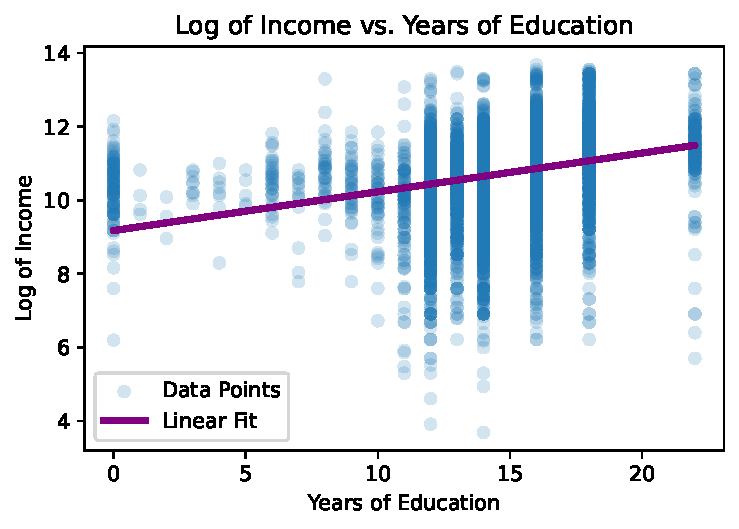
\includegraphics{mini-lesson-1_files/figure-pdf/cell-9-output-1.pdf}

\begin{enumerate}
\def\labelenumi{\arabic{enumi}.}
\setcounter{enumi}{2}
\tightlist
\item
\end{enumerate}

\begin{Shaded}
\begin{Highlighting}[]
\CommentTok{\#\# load libraries}
\ImportTok{import}\NormalTok{ statsmodels.formula.api }\ImportTok{as}\NormalTok{ smf}

\CommentTok{\#\# estimate given model }
\NormalTok{regression }\OperatorTok{=}\NormalTok{ smf.ols(}\StringTok{\textquotesingle{}lnincwage \textasciitilde{} EDUCDC + female + AGE + age\_sq + white + black + hispanic + married + NCHILD + vet\textquotesingle{}}\NormalTok{, data }\OperatorTok{=}\NormalTok{ edu\_merged\_clean).fit()}
\BuiltInTok{print}\NormalTok{(regression.summary())}
\end{Highlighting}
\end{Shaded}

\begin{verbatim}
                            OLS Regression Results                            
==============================================================================
Dep. Variable:              lnincwage   R-squared:                       0.294
Model:                            OLS   Adj. R-squared:                  0.293
Method:                 Least Squares   F-statistic:                     360.7
Date:                Fri, 31 Jan 2025   Prob (F-statistic):               0.00
Time:                        01:41:47   Log-Likelihood:                -11418.
No. Observations:                8683   AIC:                         2.286e+04
Df Residuals:                    8672   BIC:                         2.294e+04
Df Model:                          10                                         
Covariance Type:            nonrobust                                         
==============================================================================
                 coef    std err          t      P>|t|      [0.025      0.975]
------------------------------------------------------------------------------
Intercept      6.3154      0.113     56.063      0.000       6.095       6.536
EDUCDC         0.0889      0.003     26.606      0.000       0.082       0.095
female        -0.4297      0.020    -21.793      0.000      -0.468      -0.391
AGE            0.1465      0.006     26.355      0.000       0.136       0.157
age_sq        -0.0015   6.55e-05    -23.041      0.000      -0.002      -0.001
white          0.0096      0.027      0.362      0.718      -0.043       0.062
black         -0.1984      0.043     -4.621      0.000      -0.283      -0.114
hispanic      -0.0883      0.032     -2.762      0.006      -0.151      -0.026
married        0.2116      0.023      9.312      0.000       0.167       0.256
NCHILD     -5.364e-05      0.010     -0.005      0.996      -0.020       0.020
vet           -0.1387      0.051     -2.744      0.006      -0.238      -0.040
==============================================================================
Omnibus:                     2210.672   Durbin-Watson:                   1.858
Prob(Omnibus):                  0.000   Jarque-Bera (JB):             8303.702
Skew:                          -1.233   Prob(JB):                         0.00
Kurtosis:                       7.108   Cond. No.                     2.60e+04
==============================================================================

Notes:
[1] Standard Errors assume that the covariance matrix of the errors is correctly specified.
[2] The condition number is large, 2.6e+04. This might indicate that there are
strong multicollinearity or other numerical problems.
\end{verbatim}

\begin{enumerate}
\def\labelenumi{\alph{enumi}.}
\item
  According to the R\^{}2 value, the model explains 29\% of the
  variation in log wages.
\item
  An additional year of education gives an increase of 8.9\% in income,
  holding all else constant. This is statistically significant at the
  5\% significance level with a p value that is less than 0.05 but
  practically this doesn't necessarily hold true for all levels of
  education.
\end{enumerate}

For example, no children work thus a change from 2 to 3 years of
education (which would signify a toddler) then their wage should not
increase but rather stay static at 0. This would be the case all the way
until an individual reaches high school which is 12 years of schooling
at which point they are able to legally get a job and then additional
years of schooling would impact their earnings.

\begin{enumerate}
\def\labelenumi{\alph{enumi}.}
\setcounter{enumi}{2}
\tightlist
\item
  To figure out the age that gives the largest increase in \% of age,
  take the derivative of the regression with respect to age and solve
  for the variable. This gives an age of 49 that yields the highest \%
  increase in wage.
\end{enumerate}

(see calculations at end of PDF)

\begin{enumerate}
\def\labelenumi{\alph{enumi}.}
\setcounter{enumi}{3}
\item
  The model predicts that men will have higher wages, all else equal, as
  indicated by the negative value of the female coefficient of -0.4297.
  We might observe this pattern in the data because there might be bias
  against women to pay them less than their male counterparts.
\item
  Holding all else equal, being white is associated with a 0.96\%
  increase in wage. This value is not significant however because the p
  value is larger than the threshold significance level of 0.05.
\end{enumerate}

Being black, holding all else equal, is associated with a 19.8\%
decrease in wages and this value is significant because the p value is
smaller than 0.05.

\begin{enumerate}
\def\labelenumi{\arabic{enumi}.}
\setcounter{enumi}{3}
\tightlist
\item
\end{enumerate}

\begin{Shaded}
\begin{Highlighting}[]
\CommentTok{\#\# subset no high school (hsdip=0 AND coldip=0)}
\NormalTok{no\_hsd }\OperatorTok{=}\NormalTok{ edu\_merged\_clean[(edu\_merged\_clean[}\StringTok{\textquotesingle{}hsdip\textquotesingle{}}\NormalTok{] }\OperatorTok{==} \DecValTok{0}\NormalTok{) }\OperatorTok{\&}\NormalTok{ (edu\_merged\_clean[}\StringTok{\textquotesingle{}coldip\textquotesingle{}}\NormalTok{] }\OperatorTok{==}\DecValTok{0}\NormalTok{)] }

\CommentTok{\#\# fit the linear regression prediction of lnincwage vs education for hsdip=0}
\NormalTok{y\_nhs }\OperatorTok{=}\NormalTok{ no\_hsd[[}\StringTok{\textquotesingle{}lnincwage\textquotesingle{}}\NormalTok{]].values}
\NormalTok{X\_nhs }\OperatorTok{=}\NormalTok{ no\_hsd[[}\StringTok{\textquotesingle{}EDUCDC\textquotesingle{}}\NormalTok{]].values}
\NormalTok{y\_pred\_nhs }\OperatorTok{=}\NormalTok{ lm().fit(X\_nhs, y\_nhs).predict(X\_nhs)}
\end{Highlighting}
\end{Shaded}

\begin{Shaded}
\begin{Highlighting}[]
\CommentTok{\#\# subset high school diploma (hsdip=1)}
\NormalTok{hsd }\OperatorTok{=}\NormalTok{ edu\_merged\_clean[edu\_merged\_clean[}\StringTok{\textquotesingle{}hsdip\textquotesingle{}}\NormalTok{] }\OperatorTok{==} \DecValTok{1}\NormalTok{]}

\CommentTok{\#\# fit the linear regression prediction of lnincwage vs education for hsdip=0}
\NormalTok{y1 }\OperatorTok{=}\NormalTok{ hsd[[}\StringTok{\textquotesingle{}lnincwage\textquotesingle{}}\NormalTok{]].values}
\NormalTok{X1 }\OperatorTok{=}\NormalTok{ hsd[[}\StringTok{\textquotesingle{}EDUCDC\textquotesingle{}}\NormalTok{ ]].values}
\NormalTok{y\_pred\_hsd }\OperatorTok{=}\NormalTok{ lm().fit(X1, y1).predict(X1)}
\end{Highlighting}
\end{Shaded}

\begin{Shaded}
\begin{Highlighting}[]
\CommentTok{\#\# subset high school diploma (coldip=1)}
\NormalTok{col }\OperatorTok{=}\NormalTok{ edu\_merged\_clean[edu\_merged\_clean[}\StringTok{\textquotesingle{}coldip\textquotesingle{}}\NormalTok{] }\OperatorTok{==} \DecValTok{1}\NormalTok{]}

\CommentTok{\#\# fit the linear regression prediction of lnincwage vs education for hsdip=0}
\NormalTok{y2 }\OperatorTok{=}\NormalTok{ col[[}\StringTok{\textquotesingle{}lnincwage\textquotesingle{}}\NormalTok{]].values}
\NormalTok{X2 }\OperatorTok{=}\NormalTok{ col[[}\StringTok{\textquotesingle{}EDUCDC\textquotesingle{}}\NormalTok{ ]].values}
\NormalTok{y\_pred\_col }\OperatorTok{=}\NormalTok{ lm().fit(X2, y2).predict(X2)}
\end{Highlighting}
\end{Shaded}

\begin{Shaded}
\begin{Highlighting}[]
\CommentTok{\#\# graph the plot with the three separate trendlines }
\NormalTok{fig,ax }\OperatorTok{=}\NormalTok{ plt.subplots()}
\NormalTok{ax.scatter(edu\_merged\_clean[}\StringTok{\textquotesingle{}EDUCDC\textquotesingle{}}\NormalTok{], edu\_merged\_clean[}\StringTok{\textquotesingle{}lnincwage\textquotesingle{}}\NormalTok{], alpha}\OperatorTok{=}\FloatTok{0.2}\NormalTok{, s}\OperatorTok{=}\DecValTok{25}\NormalTok{, label}\OperatorTok{=}\StringTok{\textquotesingle{}Data Points\textquotesingle{}}\NormalTok{)}
\NormalTok{ax.plot(X\_nhs, y\_pred\_nhs, color}\OperatorTok{=}\StringTok{"orange"}\NormalTok{, linewidth}\OperatorTok{=}\DecValTok{3}\NormalTok{, label}\OperatorTok{=}\StringTok{\textquotesingle{}No High School Diploma\textquotesingle{}}\NormalTok{)}
\NormalTok{ax.plot(X1, y\_pred\_hsd, color}\OperatorTok{=}\StringTok{"yellow"}\NormalTok{, linewidth}\OperatorTok{=}\DecValTok{3}\NormalTok{, label}\OperatorTok{=}\StringTok{\textquotesingle{}High School Diploma\textquotesingle{}}\NormalTok{)}
\NormalTok{ax.plot(X2, y\_pred\_col, color}\OperatorTok{=}\StringTok{"green"}\NormalTok{, linewidth}\OperatorTok{=}\DecValTok{3}\NormalTok{, label}\OperatorTok{=}\StringTok{\textquotesingle{}College Diploma\textquotesingle{}}\NormalTok{)}

\NormalTok{ax.set\_xlabel(}\StringTok{"Years of Education"}\NormalTok{)}
\NormalTok{ax.set\_ylabel(}\StringTok{"Log of Income"}\NormalTok{)}
\NormalTok{ax.set\_title(}\StringTok{\textquotesingle{}Log of Income vs. Years of Education\textquotesingle{}}\NormalTok{)}
\NormalTok{ax.legend()}
\end{Highlighting}
\end{Shaded}

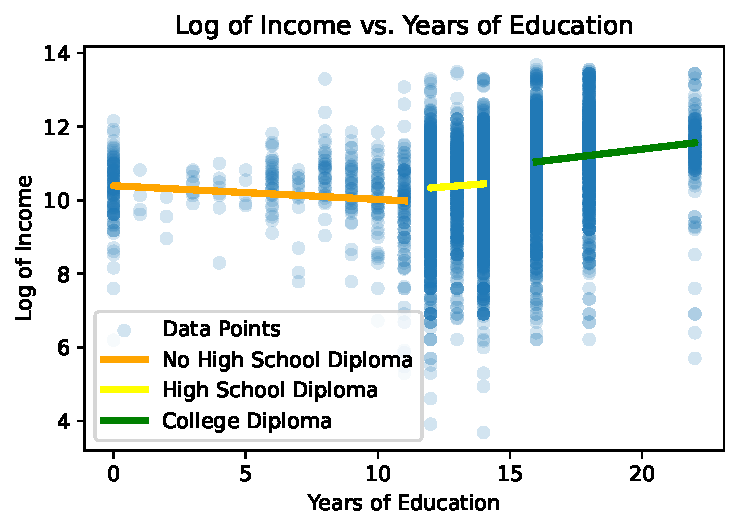
\includegraphics{mini-lesson-1_files/figure-pdf/cell-14-output-1.pdf}

\subsection{Question 5}\label{question-5}

\begin{enumerate}
\def\labelenumi{\alph{enumi}.}
\item
  The equation is
  \(ln(incwage)= \beta_{0} + \beta_{1}hsdip + \beta_{2}coldip +\beta_{3}female+\beta_{4}age+\beta_{5}age^2+\beta_{6}white+\beta_{7}black+\beta_{8}hispanic+\beta_{9}married+\beta_{10}nchild+\beta_{11}vet+\varepsilon\)
  I think this is the best possible way to explain the data because it
  allows for conditioning based on the different education levels which
  in turn are different combinations of the variables hsdip and coldip.
\item
\end{enumerate}

\begin{Shaded}
\begin{Highlighting}[]
\CommentTok{\#\# estimate this model }
\NormalTok{regression1 }\OperatorTok{=}\NormalTok{ smf.ols(}\StringTok{\textquotesingle{}lnincwage \textasciitilde{} hsdip + coldip + female + AGE + age\_sq + white + black + hispanic + married + NCHILD + vet\textquotesingle{}}\NormalTok{, data }\OperatorTok{=}\NormalTok{ edu\_merged\_clean).fit()}
\BuiltInTok{print}\NormalTok{(regression1.summary())}
\end{Highlighting}
\end{Shaded}

\begin{verbatim}
                            OLS Regression Results                            
==============================================================================
Dep. Variable:              lnincwage   R-squared:                       0.314
Model:                            OLS   Adj. R-squared:                  0.313
Method:                 Least Squares   F-statistic:                     360.2
Date:                Fri, 31 Jan 2025   Prob (F-statistic):               0.00
Time:                        01:41:48   Log-Likelihood:                -11294.
No. Observations:                8683   AIC:                         2.261e+04
Df Residuals:                    8671   BIC:                         2.270e+04
Df Model:                          11                                         
Covariance Type:            nonrobust                                         
==============================================================================
                 coef    std err          t      P>|t|      [0.025      0.975]
------------------------------------------------------------------------------
Intercept      7.2375      0.114     63.699      0.000       7.015       7.460
hsdip          0.2831      0.046      6.155      0.000       0.193       0.373
coldip         0.8867      0.047     18.718      0.000       0.794       0.980
female        -0.4317      0.019    -22.220      0.000      -0.470      -0.394
AGE            0.1371      0.006     24.872      0.000       0.126       0.148
age_sq        -0.0014   6.49e-05    -21.520      0.000      -0.002      -0.001
white          0.0288      0.026      1.093      0.274      -0.023       0.080
black         -0.1643      0.042     -3.876      0.000      -0.247      -0.081
hispanic      -0.0854      0.031     -2.714      0.007      -0.147      -0.024
married        0.1882      0.022      8.385      0.000       0.144       0.232
NCHILD         0.0053      0.010      0.526      0.599      -0.014       0.025
vet           -0.0985      0.050     -1.974      0.048      -0.196      -0.001
==============================================================================
Omnibus:                     2281.164   Durbin-Watson:                   1.868
Prob(Omnibus):                  0.000   Jarque-Bera (JB):             8620.565
Skew:                          -1.271   Prob(JB):                         0.00
Kurtosis:                       7.167   Cond. No.                     2.72e+04
==============================================================================

Notes:
[1] Standard Errors assume that the covariance matrix of the errors is correctly specified.
[2] The condition number is large, 2.72e+04. This might indicate that there are
strong multicollinearity or other numerical problems.
\end{verbatim}

\begin{enumerate}
\def\labelenumi{\alph{enumi}.}
\setcounter{enumi}{2}
\tightlist
\item
\end{enumerate}

\begin{Shaded}
\begin{Highlighting}[]
\CommentTok{\#\# predict for 22 yr old female (who is neither white, black, nor Hispanic, is not married, has no children, and is not a veteran) with a high school diploma}
\NormalTok{hs\_22\_f }\OperatorTok{=}\NormalTok{ edu\_merged\_clean.loc[(edu\_merged\_clean[}\StringTok{\textquotesingle{}AGE\textquotesingle{}}\NormalTok{] }\OperatorTok{==} \DecValTok{22}\NormalTok{) }\OperatorTok{\&}\NormalTok{ (edu\_merged\_clean[}\StringTok{\textquotesingle{}female\textquotesingle{}}\NormalTok{] }\OperatorTok{==} \DecValTok{1}\NormalTok{) }\OperatorTok{\&}\NormalTok{ (edu\_merged\_clean[}\StringTok{\textquotesingle{}hsdip\textquotesingle{}}\NormalTok{] }\OperatorTok{==} \DecValTok{1}\NormalTok{) }\OperatorTok{\&}\NormalTok{ (edu\_merged\_clean[}\StringTok{\textquotesingle{}coldip\textquotesingle{}}\NormalTok{] }\OperatorTok{==} \DecValTok{0}\NormalTok{)]}
\NormalTok{pred1 }\OperatorTok{=}\NormalTok{ regression1.get\_prediction(hs\_22\_f)}
\NormalTok{pred1.summary\_frame(alpha}\OperatorTok{=}\FloatTok{0.05}\NormalTok{)[:}\DecValTok{1}\NormalTok{]}

\ImportTok{import}\NormalTok{ math }
\NormalTok{math.exp(}\FloatTok{9.428}\NormalTok{)}

\CommentTok{\#\# predict but with college diploma}
\NormalTok{col\_22\_f }\OperatorTok{=}\NormalTok{ edu\_merged\_clean.loc[(edu\_merged\_clean[}\StringTok{\textquotesingle{}AGE\textquotesingle{}}\NormalTok{] }\OperatorTok{==} \DecValTok{22}\NormalTok{) }\OperatorTok{\&}\NormalTok{ (edu\_merged\_clean[}\StringTok{\textquotesingle{}female\textquotesingle{}}\NormalTok{] }\OperatorTok{==} \DecValTok{1}\NormalTok{) }\OperatorTok{\&}\NormalTok{ (edu\_merged\_clean[}\StringTok{\textquotesingle{}hsdip\textquotesingle{}}\NormalTok{] }\OperatorTok{==} \DecValTok{0}\NormalTok{) }\OperatorTok{\&}\NormalTok{ (edu\_merged\_clean[}\StringTok{\textquotesingle{}coldip\textquotesingle{}}\NormalTok{] }\OperatorTok{==} \DecValTok{1}\NormalTok{)]}
\NormalTok{pred2 }\OperatorTok{=}\NormalTok{ regression1.get\_prediction(col\_22\_f)}
\NormalTok{pred2.summary\_frame(alpha}\OperatorTok{=}\FloatTok{0.05}\NormalTok{)[:}\DecValTok{1}\NormalTok{]}

\NormalTok{math.exp(}\FloatTok{9.946}\NormalTok{)}
\end{Highlighting}
\end{Shaded}

\begin{verbatim}
20868.580886763528
\end{verbatim}

For a 22 year old female (who is neither white, black, nor Hispanic, is
not married, has no children, and is not a veteran) with a high school
diploma then their expected wages, will be e\^{}9.428 which is \$12,431.
For this same individual with a college degree their wage is equal to
e\^{}9.946 which is \$20,868.

\begin{enumerate}
\def\labelenumi{\alph{enumi}.}
\setcounter{enumi}{3}
\item
  Looking a the model, there is a coefficient of 0.8867 for the college
  diploma term which means that holding all else equal there is on
  average about an 89\% increase in wages for a person with a college
  degree compared to someone who does not have one. This is
  statistically significant at the 5\% significance level.
\item
  Given the evidence, I would advise the President to pursue legislation
  to expand access to college education since it seems to have a large
  and significant effect on wages even when holding other variables like
  gender, age, race, married status, and number of children fixed.
\item
  This new model explains 31\% of the variation that's observed in log
  income which is slightly higher than the previous model. The previous
  model explained 29.3\%.
\item
  I'm pretty confident in my predictions because the increase in log
  wages is significant for individuals with a degree and the model
  explains over 30\% of the variation in log wages that is observed in
  the data. This is pretty good considering the complexity of the
  relationship that we are trying to explain and the use of various
  predictors to try and control for other potential influences.
\end{enumerate}

\subsection{Question 6}\label{question-6}

\begin{Shaded}
\begin{Highlighting}[]
\CommentTok{\#\# library}
\ImportTok{from}\NormalTok{ sklearn.preprocessing }\ImportTok{import}\NormalTok{ SplineTransformer}
\ImportTok{from}\NormalTok{ sklearn.linear\_model }\ImportTok{import}\NormalTok{ LinearRegression}

\CommentTok{\#\# prepare variables}
\NormalTok{X\_age }\OperatorTok{=}\NormalTok{ edu\_merged\_clean[[}\StringTok{\textquotesingle{}AGE\textquotesingle{}}\NormalTok{]]}
\NormalTok{X\_hsdip }\OperatorTok{=}\NormalTok{ edu\_merged\_clean[[}\StringTok{\textquotesingle{}hsdip\textquotesingle{}}\NormalTok{]]}
\NormalTok{X\_coldip }\OperatorTok{=}\NormalTok{ edu\_merged\_clean[[}\StringTok{\textquotesingle{}coldip\textquotesingle{}}\NormalTok{]]}
\NormalTok{X\_fem }\OperatorTok{=}\NormalTok{ edu\_merged\_clean[[}\StringTok{\textquotesingle{}female\textquotesingle{}}\NormalTok{]]}
\NormalTok{X\_white }\OperatorTok{=}\NormalTok{ edu\_merged\_clean[[}\StringTok{\textquotesingle{}white\textquotesingle{}}\NormalTok{]]}
\NormalTok{X\_black }\OperatorTok{=}\NormalTok{ edu\_merged\_clean[[}\StringTok{\textquotesingle{}black\textquotesingle{}}\NormalTok{]]}
\NormalTok{X\_hispanic }\OperatorTok{=}\NormalTok{ edu\_merged\_clean[[}\StringTok{\textquotesingle{}hispanic\textquotesingle{}}\NormalTok{]]}
\NormalTok{X\_married }\OperatorTok{=}\NormalTok{ edu\_merged\_clean[[}\StringTok{\textquotesingle{}married\textquotesingle{}}\NormalTok{]]}
\NormalTok{X\_nchild }\OperatorTok{=}\NormalTok{ edu\_merged\_clean[[}\StringTok{\textquotesingle{}NCHILD\textquotesingle{}}\NormalTok{]]}
\NormalTok{X\_vet }\OperatorTok{=}\NormalTok{ edu\_merged\_clean[[}\StringTok{\textquotesingle{}vet\textquotesingle{}}\NormalTok{]]}
\NormalTok{y }\OperatorTok{=}\NormalTok{ edu\_merged\_clean[}\StringTok{\textquotesingle{}lnincwage\textquotesingle{}}\NormalTok{]}

\CommentTok{\#\# knots for the age variable}
\NormalTok{knots }\OperatorTok{=}\NormalTok{ np.array([}\DecValTok{18}\NormalTok{, }\DecValTok{65}\NormalTok{]).reshape(}\OperatorTok{{-}}\DecValTok{1}\NormalTok{, }\DecValTok{1}\NormalTok{)}

\CommentTok{\#\# spline transformer}
\NormalTok{spline\_transformer }\OperatorTok{=}\NormalTok{ SplineTransformer(degree}\OperatorTok{=}\DecValTok{3}\NormalTok{, knots }\OperatorTok{=}\NormalTok{ knots, include\_bias }\OperatorTok{=} \VariableTok{False}\NormalTok{)}

\CommentTok{\#\# transofrm age into spline functions}
\NormalTok{X\_splines }\OperatorTok{=}\NormalTok{ spline\_transformer.fit\_transform(X\_age)}

\CommentTok{\#\# combine with controls }
\NormalTok{X }\OperatorTok{=}\NormalTok{ np.hstack([X\_splines, X\_hsdip, X\_coldip, X\_fem, X\_white, X\_black, X\_hispanic, X\_married, X\_nchild, X\_vet])}

\CommentTok{\#\# fit linear reg model }
\NormalTok{final }\OperatorTok{=}\NormalTok{ LinearRegression()}
\NormalTok{final.fit(X,y)}

\CommentTok{\#\# print intercept }
\BuiltInTok{print}\NormalTok{(}\StringTok{\textquotesingle{}Intercept:\textquotesingle{}}\NormalTok{, final.intercept\_)}

\CommentTok{\#\# combine coefficient names }
\NormalTok{spline\_columns }\OperatorTok{=}\NormalTok{ [}\SpecialStringTok{f"spline\_}\SpecialCharTok{\{}\NormalTok{i}\SpecialCharTok{\}}\SpecialStringTok{"} \ControlFlowTok{for}\NormalTok{ i }\KeywordTok{in} \BuiltInTok{range}\NormalTok{(X\_splines.shape[}\DecValTok{1}\NormalTok{])]}
\NormalTok{all\_columns }\OperatorTok{=}\NormalTok{ spline\_columns }\OperatorTok{+}\NormalTok{ [}\StringTok{\textquotesingle{}hsdip\textquotesingle{}}\NormalTok{] }\OperatorTok{+}\NormalTok{ [}\StringTok{\textquotesingle{}coldip\textquotesingle{}}\NormalTok{] }\OperatorTok{+}\NormalTok{ [}\StringTok{\textquotesingle{}female\textquotesingle{}}\NormalTok{] }\OperatorTok{+}\NormalTok{ [}\StringTok{\textquotesingle{}white\textquotesingle{}}\NormalTok{] }\OperatorTok{+}\NormalTok{ [}\StringTok{\textquotesingle{}black\textquotesingle{}}\NormalTok{] }\OperatorTok{+}\NormalTok{ [}\StringTok{\textquotesingle{}hispanic\textquotesingle{}}\NormalTok{] }\OperatorTok{+}\NormalTok{ [}\StringTok{\textquotesingle{}married\textquotesingle{}}\NormalTok{] }\OperatorTok{+}\NormalTok{ [}\StringTok{\textquotesingle{}NCHILD\textquotesingle{}}\NormalTok{] }\OperatorTok{+}\NormalTok{ [}\StringTok{\textquotesingle{}vet\textquotesingle{}}\NormalTok{]}
\NormalTok{coefficients }\OperatorTok{=}\NormalTok{ pd.Series(final.coef\_, index}\OperatorTok{=}\NormalTok{all\_columns)}
\BuiltInTok{print}\NormalTok{(}\StringTok{"Coefficients:"}\NormalTok{)}
\BuiltInTok{print}\NormalTok{(coefficients)}

\CommentTok{\#\# get adj r\^{}2}
\CommentTok{\# Calculate R\^{}2}
\NormalTok{r\_squared }\OperatorTok{=}\NormalTok{ final.score(X, y)}

\NormalTok{n }\OperatorTok{=} \BuiltInTok{len}\NormalTok{(y)  }
\NormalTok{p }\OperatorTok{=}\NormalTok{ X\_splines.shape[}\DecValTok{1}\NormalTok{]  }
\NormalTok{adjusted\_r\_squared }\OperatorTok{=} \DecValTok{1} \OperatorTok{{-}}\NormalTok{ ((}\DecValTok{1} \OperatorTok{{-}}\NormalTok{ r\_squared) }\OperatorTok{*}\NormalTok{ (n }\OperatorTok{{-}} \DecValTok{1}\NormalTok{)) }\OperatorTok{/}\NormalTok{ (n }\OperatorTok{{-}}\NormalTok{ p }\OperatorTok{{-}} \DecValTok{1}\NormalTok{)}
\BuiltInTok{print}\NormalTok{(}\StringTok{"Adjusted R{-}squared:"}\NormalTok{, adjusted\_r\_squared)}
\end{Highlighting}
\end{Shaded}

\begin{verbatim}
Intercept: 14.331135251571602
Coefficients:
spline_0   -19.476711
spline_1    -1.780260
spline_2    -5.272285
hsdip        0.273681
coldip       0.854378
female      -0.428941
white        0.024746
black       -0.166548
hispanic    -0.093290
married      0.181026
NCHILD       0.005171
vet         -0.089764
dtype: float64
Adjusted R-squared: 0.32122736547279296
\end{verbatim}

The adjusted R\^{}2 for this model is 0.321

\begin{enumerate}
\def\labelenumi{\alph{enumi}.}
\setcounter{enumi}{1}
\item
  This adjusted R\^{}2 is different from the previous model which was
  0.313. These are different because the spline is a different model
  that allows for more flexibility than a regular linear regression so
  it would make sense that it's ability to explain variation in the y
  value of the data changes.
\item
  skip
\item
  Given the previous spline models with knots at 24 and 55, the values
  of the predictions for a female with a college diploma would be
  different because with a spline you are essentially creating mini
  models that you then stich together (at the knots) smoothly. This
  allows for more prediction accuracy because the splines behave like
  linear regression functions but have more flexibility, and therefore
  can better explain the variation in the data better than a regular OLS
  model. This is what we saw in the slightly higher adjusted R\^{}2
  value.
\end{enumerate}




\end{document}
